\documentclass{standalone}
\usepackage{tikz}
\usetikzlibrary{patterns, positioning}
\usepackage[sfdefault]{ClearSans} %% option 'sfdefault' activates Clear Sans as the default text font
\usepackage[T1]{fontenc}

\begin{document}
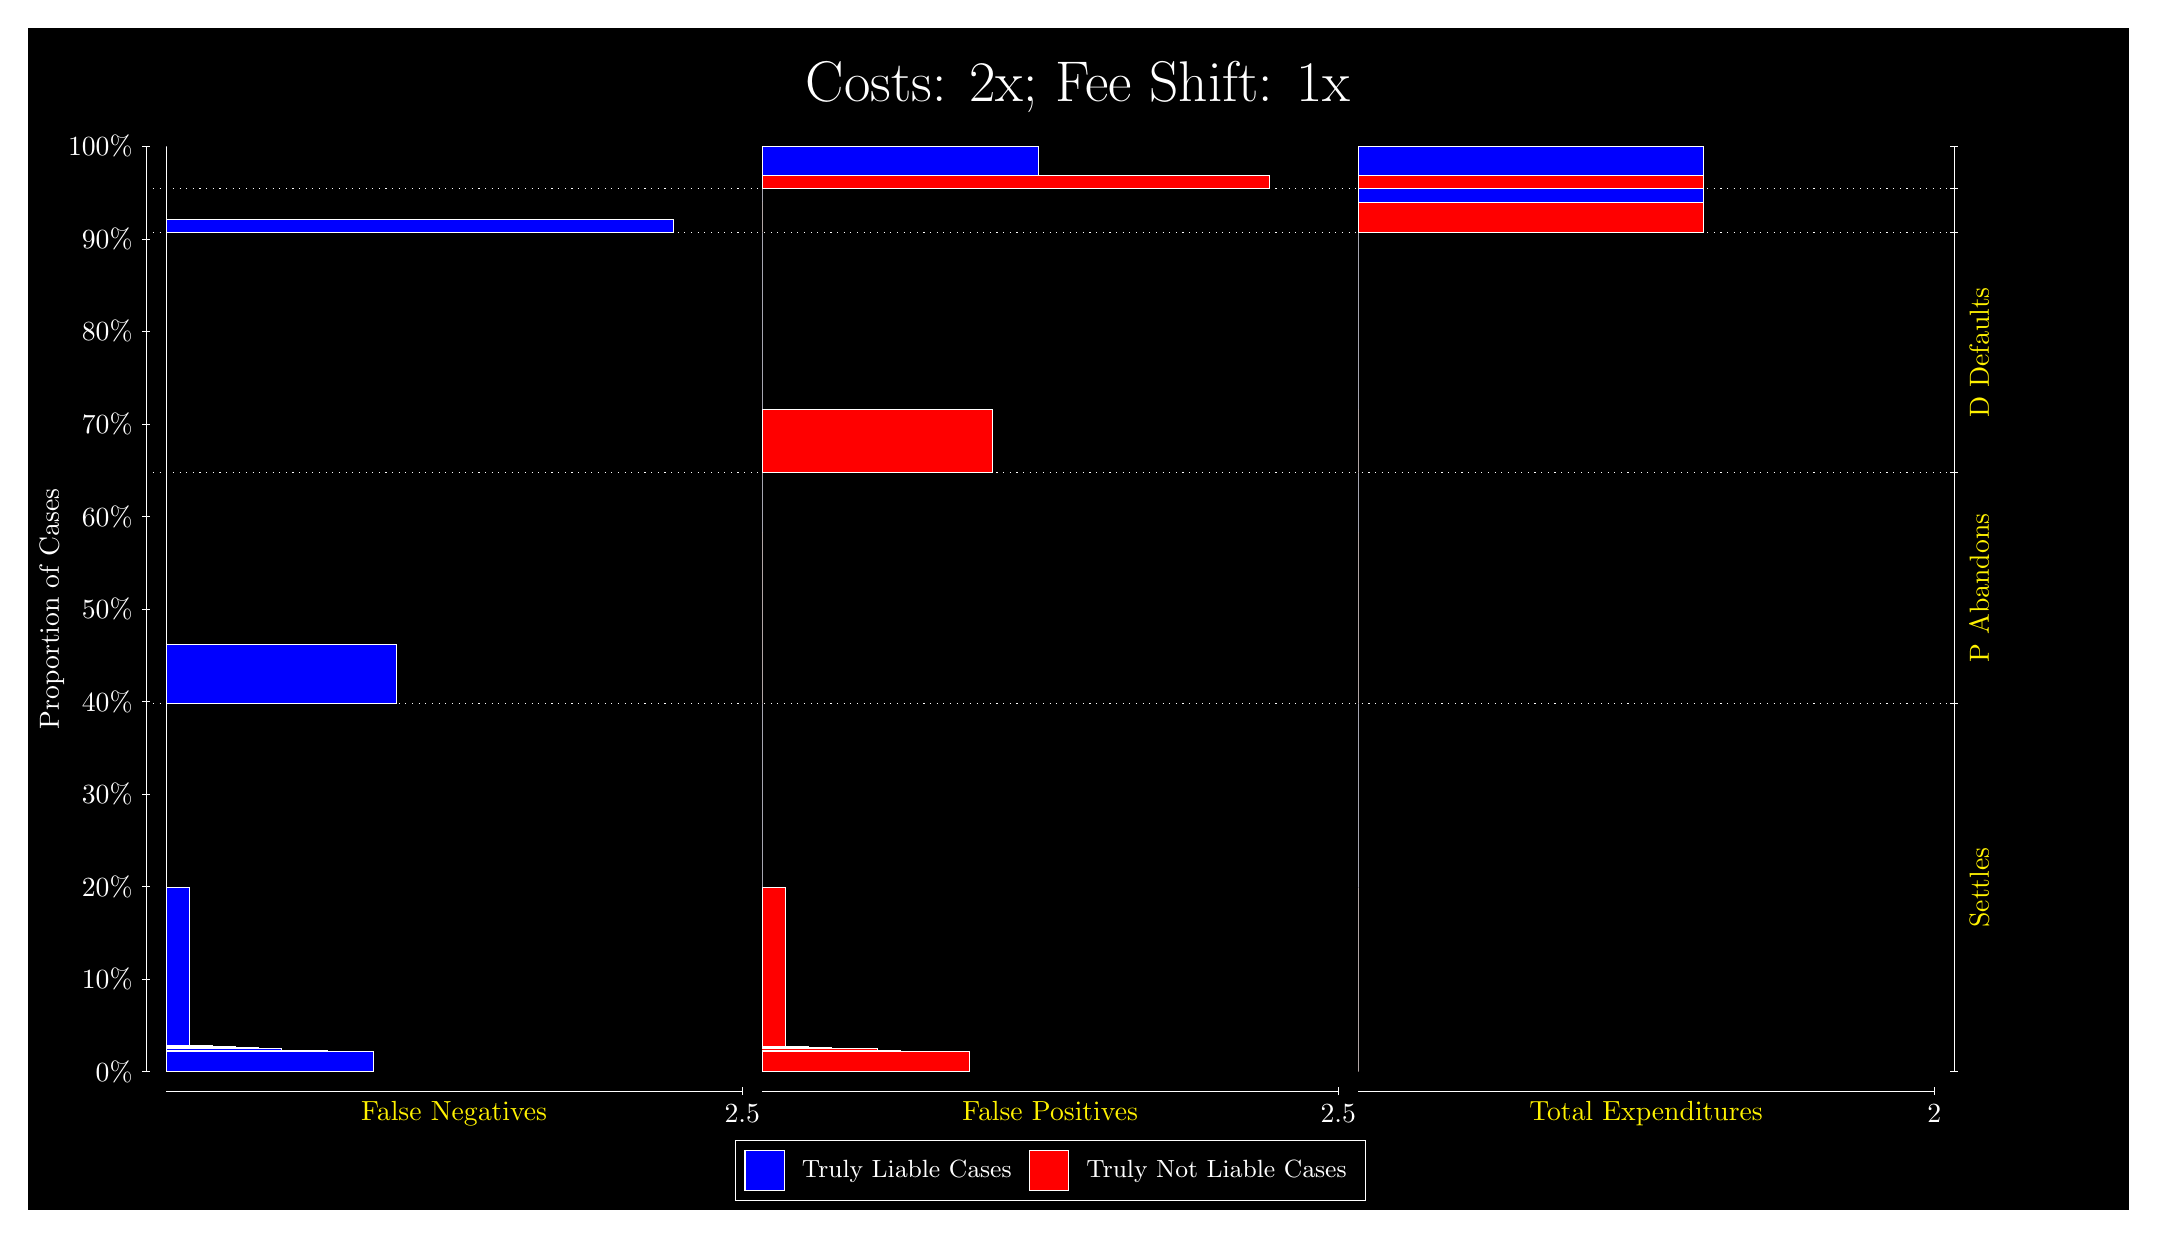
\begin{tikzpicture}
\draw[fill=black] (0,0) rectangle (26.667,15);
\draw[text=white] (0,13.5) rectangle (26.667,15) node[midway] {\huge Costs: 2x; Fee Shift: 1x};
\draw[white, very thin] (1.5,1.75) -- (1.5,13.5);
\node[rotate=90, text=white, anchor=center] at (0.3, 7.625) {Proportion of Cases};
\draw[white, very thin] (1.45,1.75) -- (1.55,1.75);
\node[text=white, anchor=east] at (1.45, 1.75) {0\%};
\draw[white, very thin] (1.45,2.925) -- (1.55,2.925);
\node[text=white, anchor=east] at (1.45, 2.925) {10\%};
\draw[white, very thin] (1.45,4.1) -- (1.55,4.1);
\node[text=white, anchor=east] at (1.45, 4.1) {20\%};
\draw[white, very thin] (1.45,5.275) -- (1.55,5.275);
\node[text=white, anchor=east] at (1.45, 5.275) {30\%};
\draw[white, very thin] (1.45,6.45) -- (1.55,6.45);
\node[text=white, anchor=east] at (1.45, 6.45) {40\%};
\draw[white, very thin] (1.45,7.625) -- (1.55,7.625);
\node[text=white, anchor=east] at (1.45, 7.625) {50\%};
\draw[white, very thin] (1.45,8.8) -- (1.55,8.8);
\node[text=white, anchor=east] at (1.45, 8.8) {60\%};
\draw[white, very thin] (1.45,9.975) -- (1.55,9.975);
\node[text=white, anchor=east] at (1.45, 9.975) {70\%};
\draw[white, very thin] (1.45,11.15) -- (1.55,11.15);
\node[text=white, anchor=east] at (1.45, 11.15) {80\%};
\draw[white, very thin] (1.45,12.325) -- (1.55,12.325);
\node[text=white, anchor=east] at (1.45, 12.325) {90\%};
\draw[white, very thin] (1.45,13.5) -- (1.55,13.5);
\node[text=white, anchor=east] at (1.45, 13.5) {100\%};

\draw[white, very thin] (24.457,1.75) -- (24.457,13.5);
\draw[white, very thin] (24.407,1.75) -- (24.507,1.75);
\node[anchor=west] at (24.407, 1.75) {};
\draw[white, very thin] (24.407,6.4252) -- (24.507,6.4252);
\node[anchor=west] at (24.407, 6.4252) {};
\draw[white, very thin] (24.407,9.3554) -- (24.507,9.3554);
\node[anchor=west] at (24.407, 9.3554) {};
\draw[white, very thin] (24.407,12.406) -- (24.507,12.406);
\node[anchor=west] at (24.407, 12.406) {};
\draw[white, very thin] (24.407,12.964) -- (24.507,12.964);
\node[anchor=west] at (24.407, 12.964) {};
\draw[white, very thin] (24.407,13.5) -- (24.507,13.5);
\node[anchor=west] at (24.407, 13.5) {};

\draw[white, very thin, fill=blue] (1.75,1.75) rectangle (4.3848,2.0101);
\draw[white, very thin, fill=blue] (1.75,2.0101) rectangle (4.092,2.0125);
\draw[white, very thin, fill=blue] (1.75,2.0125) rectangle (3.7993,2.0154);
\draw[white, very thin, fill=blue] (1.75,2.0154) rectangle (3.5065,2.0179);
\draw[white, very thin, fill=blue] (1.75,2.0179) rectangle (3.5065,2.0184);
\draw[white, very thin, fill=blue] (1.75,2.0184) rectangle (3.2138,2.042);
\draw[white, very thin, fill=blue] (1.75,2.042) rectangle (2.921,2.0534);
\draw[white, very thin, fill=blue] (1.75,2.0534) rectangle (2.6283,2.066);
\draw[white, very thin, fill=blue] (1.75,2.066) rectangle (2.3355,2.0792);
\draw[white, very thin, fill=blue] (1.75,2.0792) rectangle (2.0428,4.088);
\draw[white, very thin, fill=red] (1.75,4.088) rectangle (1.75,6.4252);
\draw[white, very thin, fill=blue] (1.75,6.4252) rectangle (4.6775,7.1807);
\draw[white, very thin, fill=red] (1.75,7.1807) rectangle (1.75,9.3554);
\draw[white, very thin, fill=red] (1.75,9.3554) rectangle (1.75,10.161);
\draw[white, very thin, fill=blue] (1.75,10.161) rectangle (1.75,12.406);
\draw[white, very thin, fill=blue] (1.75,12.406) rectangle (8.1906,12.576);
\draw[white, very thin, fill=red] (1.75,12.576) rectangle (1.75,12.964);
\draw[white, very thin, fill=red] (1.75,12.964) rectangle (1.75,13.134);
\draw[white, very thin, fill=blue] (1.75,13.134) rectangle (1.75,13.5);
\draw[white, very thin, fill=red] (9.3189,1.75) rectangle (11.954,2.006);
\draw[white, very thin, fill=red] (9.3189,2.006) rectangle (11.661,2.0094);
\draw[white, very thin, fill=red] (9.3189,2.0094) rectangle (11.368,2.013);
\draw[white, very thin, fill=red] (9.3189,2.013) rectangle (11.075,2.0164);
\draw[white, very thin, fill=red] (9.3189,2.0164) rectangle (10.783,2.0394);
\draw[white, very thin, fill=red] (9.3189,2.0394) rectangle (10.49,2.0398);
\draw[white, very thin, fill=red] (9.3189,2.0398) rectangle (10.49,2.049);
\draw[white, very thin, fill=red] (9.3189,2.049) rectangle (10.197,2.0585);
\draw[white, very thin, fill=red] (9.3189,2.0585) rectangle (9.9044,2.0675);
\draw[white, very thin, fill=red] (9.3189,2.0675) rectangle (9.6116,4.0871);
\draw[white, very thin, fill=blue] (9.3189,4.0871) rectangle (9.3189,6.4252);
\draw[white, very thin, fill=red] (9.3189,6.4252) rectangle (9.3189,8.5999);
\draw[white, very thin, fill=blue] (9.3189,8.5999) rectangle (9.3189,9.3554);
\draw[white, very thin, fill=red] (9.3189,9.3554) rectangle (12.246,10.161);
\draw[white, very thin, fill=blue] (9.3189,10.161) rectangle (9.3189,12.406);
\draw[white, very thin, fill=red] (9.3189,12.406) rectangle (9.3189,12.795);
\draw[white, very thin, fill=blue] (9.3189,12.795) rectangle (9.3189,12.964);
\draw[white, very thin, fill=red] (9.3189,12.964) rectangle (15.759,13.134);
\draw[white, very thin, fill=blue] (9.3189,13.134) rectangle (12.832,13.5);
\draw[white, very thin, fill=red] (16.888,1.75) rectangle (16.888,4.0871);
\draw[white, very thin, fill=blue] (16.888,4.0871) rectangle (16.888,6.4252);
\draw[white, very thin, fill=red] (16.888,6.4252) rectangle (16.888,8.5999);
\draw[white, very thin, fill=blue] (16.888,8.5999) rectangle (16.888,9.3554);
\draw[white, very thin, fill=red] (16.888,9.3554) rectangle (16.888,10.161);
\draw[white, very thin, fill=blue] (16.888,10.161) rectangle (16.888,12.406);
\draw[white, very thin, fill=red] (16.888,12.406) rectangle (21.279,12.795);
\draw[white, very thin, fill=blue] (16.888,12.795) rectangle (21.279,12.964);
\draw[white, very thin, fill=red] (16.888,12.964) rectangle (21.279,13.134);
\draw[white, very thin, fill=blue] (16.888,13.134) rectangle (21.279,13.5);
\draw[white, dotted] (1.5,6.4252) -- (24.457,6.4252);
\draw[white, dotted] (1.5,9.3554) -- (24.457,9.3554);
\draw[white, dotted] (1.5,12.406) -- (24.457,12.406);
\draw[white, dotted] (1.5,12.964) -- (24.457,12.964);
\draw[white, very thin] (1.75,1.5) -- (9.0689,1.5);
\node[text=yellow, anchor=north] at (5.4094, 1.5) {False Negatives};
\draw[white, very thin] (9.0689,1.45) -- (9.0689,1.55);
\node[text=white, anchor=north] at (9.0689, 1.45) {2.5};

\draw[white, very thin] (9.3189,1.5) -- (16.638,1.5);
\node[text=yellow, anchor=north] at (12.978, 1.5) {False Positives};
\draw[white, very thin] (16.638,1.45) -- (16.638,1.55);
\node[text=white, anchor=north] at (16.638, 1.45) {2.5};

\draw[white, very thin] (16.888,1.5) -- (24.207,1.5);
\node[text=yellow, anchor=north] at (20.547, 1.5) {Total Expenditures};
\draw[white, very thin] (24.207,1.45) -- (24.207,1.55);
\node[text=white, anchor=north] at (24.207, 1.45) {2};

\node[text=yellow, centered, rotate=90] at (24.777, 4.0876) {Settles};
\node[text=yellow, centered, rotate=90] at (24.777, 7.8903) {P Abandons};
\node[text=yellow, centered, rotate=90] at (24.777, 10.881) {D Defaults};



\draw (12.978300999999998,1.5) node[draw=none] (baseCoordinate) {};
\begin{scope}[align=center]
        \matrix[scale=0.5, draw=white, below=0.5cm of baseCoordinate, nodes={draw}, column sep=0.1cm]{
            \node[rectangle, draw, minimum width=0.5cm, minimum height=0.5cm, fill=blue] {}; &
            \node[draw=none, font=\small, text=white] (B) {Truly Liable Cases}; &
            \node[rectangle, draw, minimum width=0.5cm, minimum height=0.5cm, fill=red] {}; &
            \node[draw=none, font=\small, text=white] (B) {Truly Not Liable Cases}; \\
            };
\end{scope}

\end{tikzpicture}
\end{document}